\graphicspath{{./figures}}

\begin{figure}[!htb]
  \begin{minipage}{.45\textwidth}
    \centering
    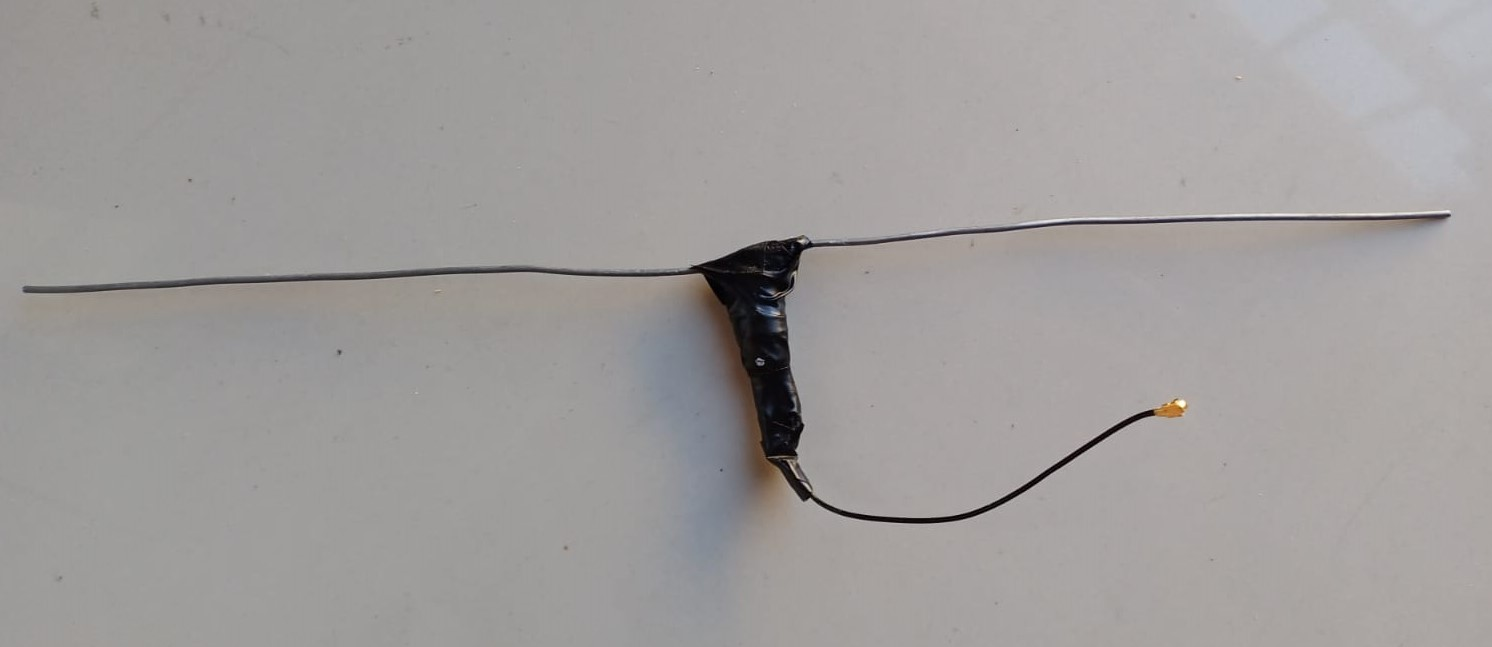
\includegraphics[width=0.9\linewidth]{pqAntenna}
    \caption{PQ Unit Antenna Implementation}
    \label{fig:pqAntenna}
  \end{minipage}
  \begin{minipage}{.49\textwidth}
    \centering
    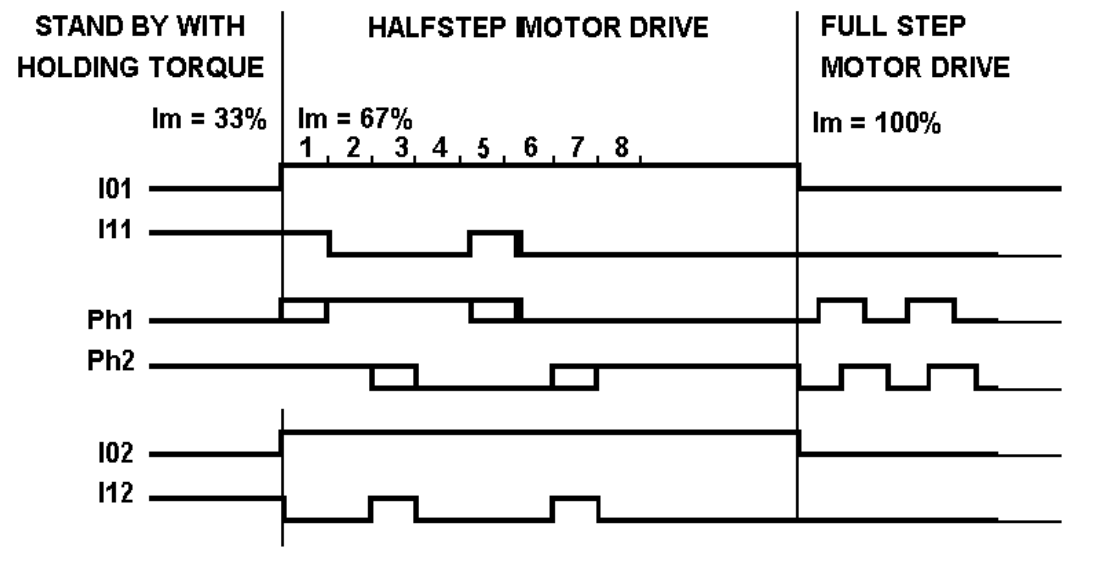
\includegraphics[width=0.98\linewidth]{stepperTiming}
    \caption{Stepper Motor Timing Diagram \cite{datasheet-L6219}}
    \label{fig:stepperTiming}
  \end{minipage}
\end{figure}

\section{Software}
All code is available at \url{https://github.com/gvcallen/pqcom/tree/main/code}.

\subsection{Mount Control}
The motors were setup in half-stepping mode, as shown in Figure \ref{fig:stepperTiming}, implemented using an array. Since both axes on the mount are dependent (see Figure \ref{fig:antennaMount}), the two-axis mount requires some relatively involved control. Elevational variation is straight-forward, as the azimuthal motor (controlled by Gear C) can be held fixed, and the elevation motor (Gear D) stepped accordingly. For azimuthal variation, if the elevation motor is held fixed, rotating the azimuthal motor causes the mount to also change in elevation, which must be compensated for (demonstrated in Appendix \ref{sec:appendix_mount_rotation}). The formulae to do this can be found in Appendix \ref{sec:appendix_mount_control}. To smoothly step both motors simultaneously, speeds are then set according to the ratio of the number of azimuthal and elevation motor steps to do.

\subsection{Pointing}
A small library titled \textit{wgs84} was used for the Mercator projection, with Cape Town as the origin. This allows a pointing vector to be determined, which is passed as the mount's boresight (where it is converted to azimuth-elevation co-ordinates). Unfortunately, the IMU (MPU-9250) was found to be counterfeit and lacked a magnetometer. The constraint was therefore made that a dead-reckoning fix to face magnetic north will be done. The angle between the zero sensor and magnetic north was therefore used as a reference input.

\subsection{Radio and GPS}
Existing Arduino libraries \textit{RadioLib} and \textit{TinyGPSPlus} were initially used for communication with the LoRa module and GPS module respectively. It was later found, however, that \textit{RadioLib} was too large in program size for the Atmega328, and it was therefore replaced with \textit{LoRaLib}, a smaller alternative.